\documentclass[a4paper, 12pt]{article}
\usepackage{titling}
\usepackage{array}
\usepackage{booktabs}
\usepackage{enumitem}
\usepackage{graphicx}
\usepackage{subfigure}
\usepackage{hyperref}
\usepackage{amssymb}
\usepackage{listings}
\setlength{\heavyrulewidth}{1.5pt}
\setlength{\abovetopsep}{4pt}
\setlength{\parindent}{0pt}
\graphicspath{{.}}

\usepackage[margin=1in]{geometry}

% Must be after geometry
\usepackage{fancyhdr}
\pagestyle{fancy}
\fancyhf{}
\rhead{ECTA Homework 2}
\cfoot{\thepage}

\setlength{\droptitle}{-5em}

\title{Evolutionary Computation Theory and Application  \\
				Assignment 2: Traveling Salesman Problem}
\author{Arun Prabhu, Dharmin B.}
\date{\today{}}

\begin{document}

\maketitle


\section{Solution}

\begin{table} [h!]
	  \centering
    \begin{tabular}{|l|c|}
    \hline
    \textbf{Parameter} & \textbf{Value}   \\\hline
    Population size & 100 \\\hline
    Crossover Rates &  0.01, 0.1, 0.99, \textbf{0.98}\\\hline
    Mutation Rates & 0.01, 0.1, 0.99, \textbf{0.25}\\\hline
    Repetitions & 30 \\\hline
    Generations & 1000 \\\hline
    Average best fitness		 & 58.8038 \\\hline
    Best fitness & 53.6009 \\\hline
    \end{tabular}
\caption{Parameters for Experiments}
\label{table:defparams}
\end{table}

\begin{table}[h!]
    \centering
    \label{tab:label}
    \begin{tabular}{|l|c|}\hline
        \textbf{Parameter} & \textbf{Value} \\\hline
        Population size & 100 \\\hline
        Fitness & 50.7048 \\\hline
        Generations & 3000 \\\hline
        Crossover rate & 0.99 \\\hline
        Mutation rate & 0.1 \\\hline
    \end{tabular}
    \caption{Parameters for Absolute best result}
\end{table}
\newpage
\section{Results}

\begin{figure}[h!]
  \centering
  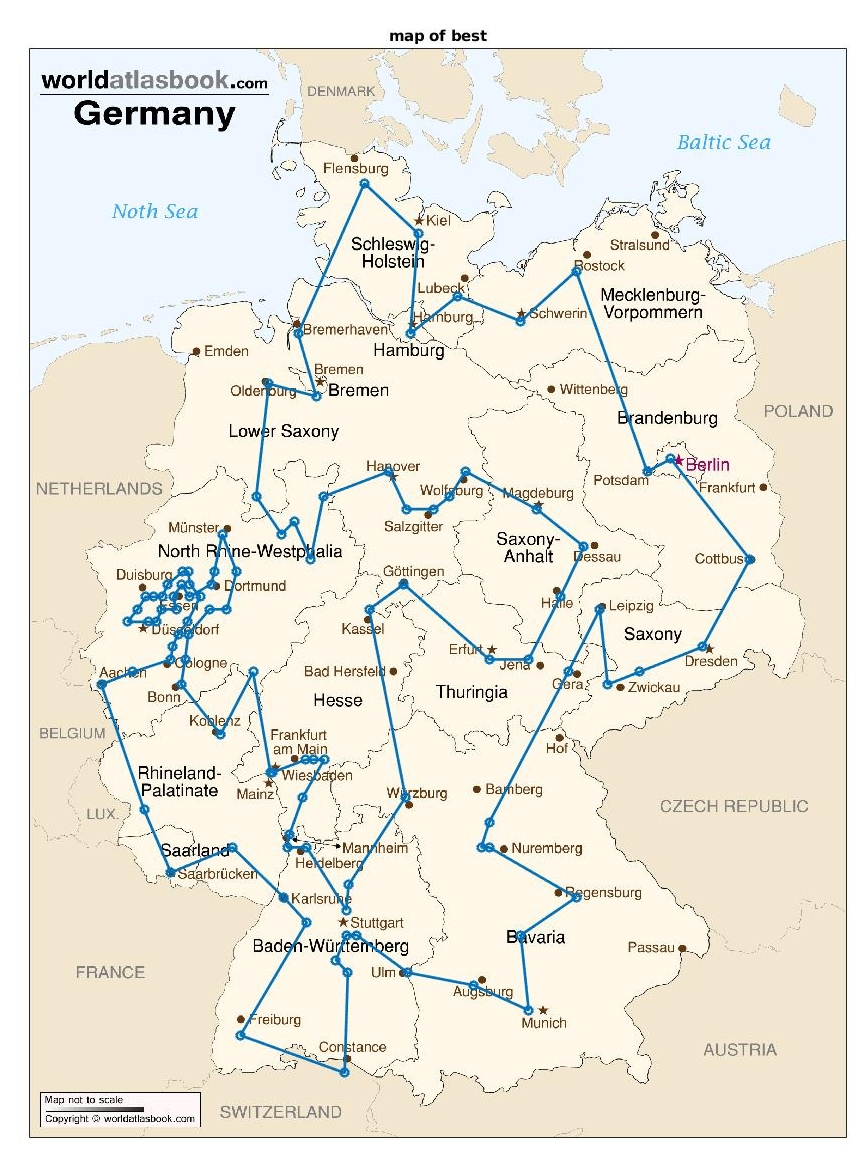
\includegraphics[width=1.0\textwidth]{images/BestPath.jpg}
    \caption{Absolute best map \label{fig:xxx1}}
\end{figure}

\newpage
\subsection{Different mutation rates}

\begin{figure}[ht!]
	\centering
	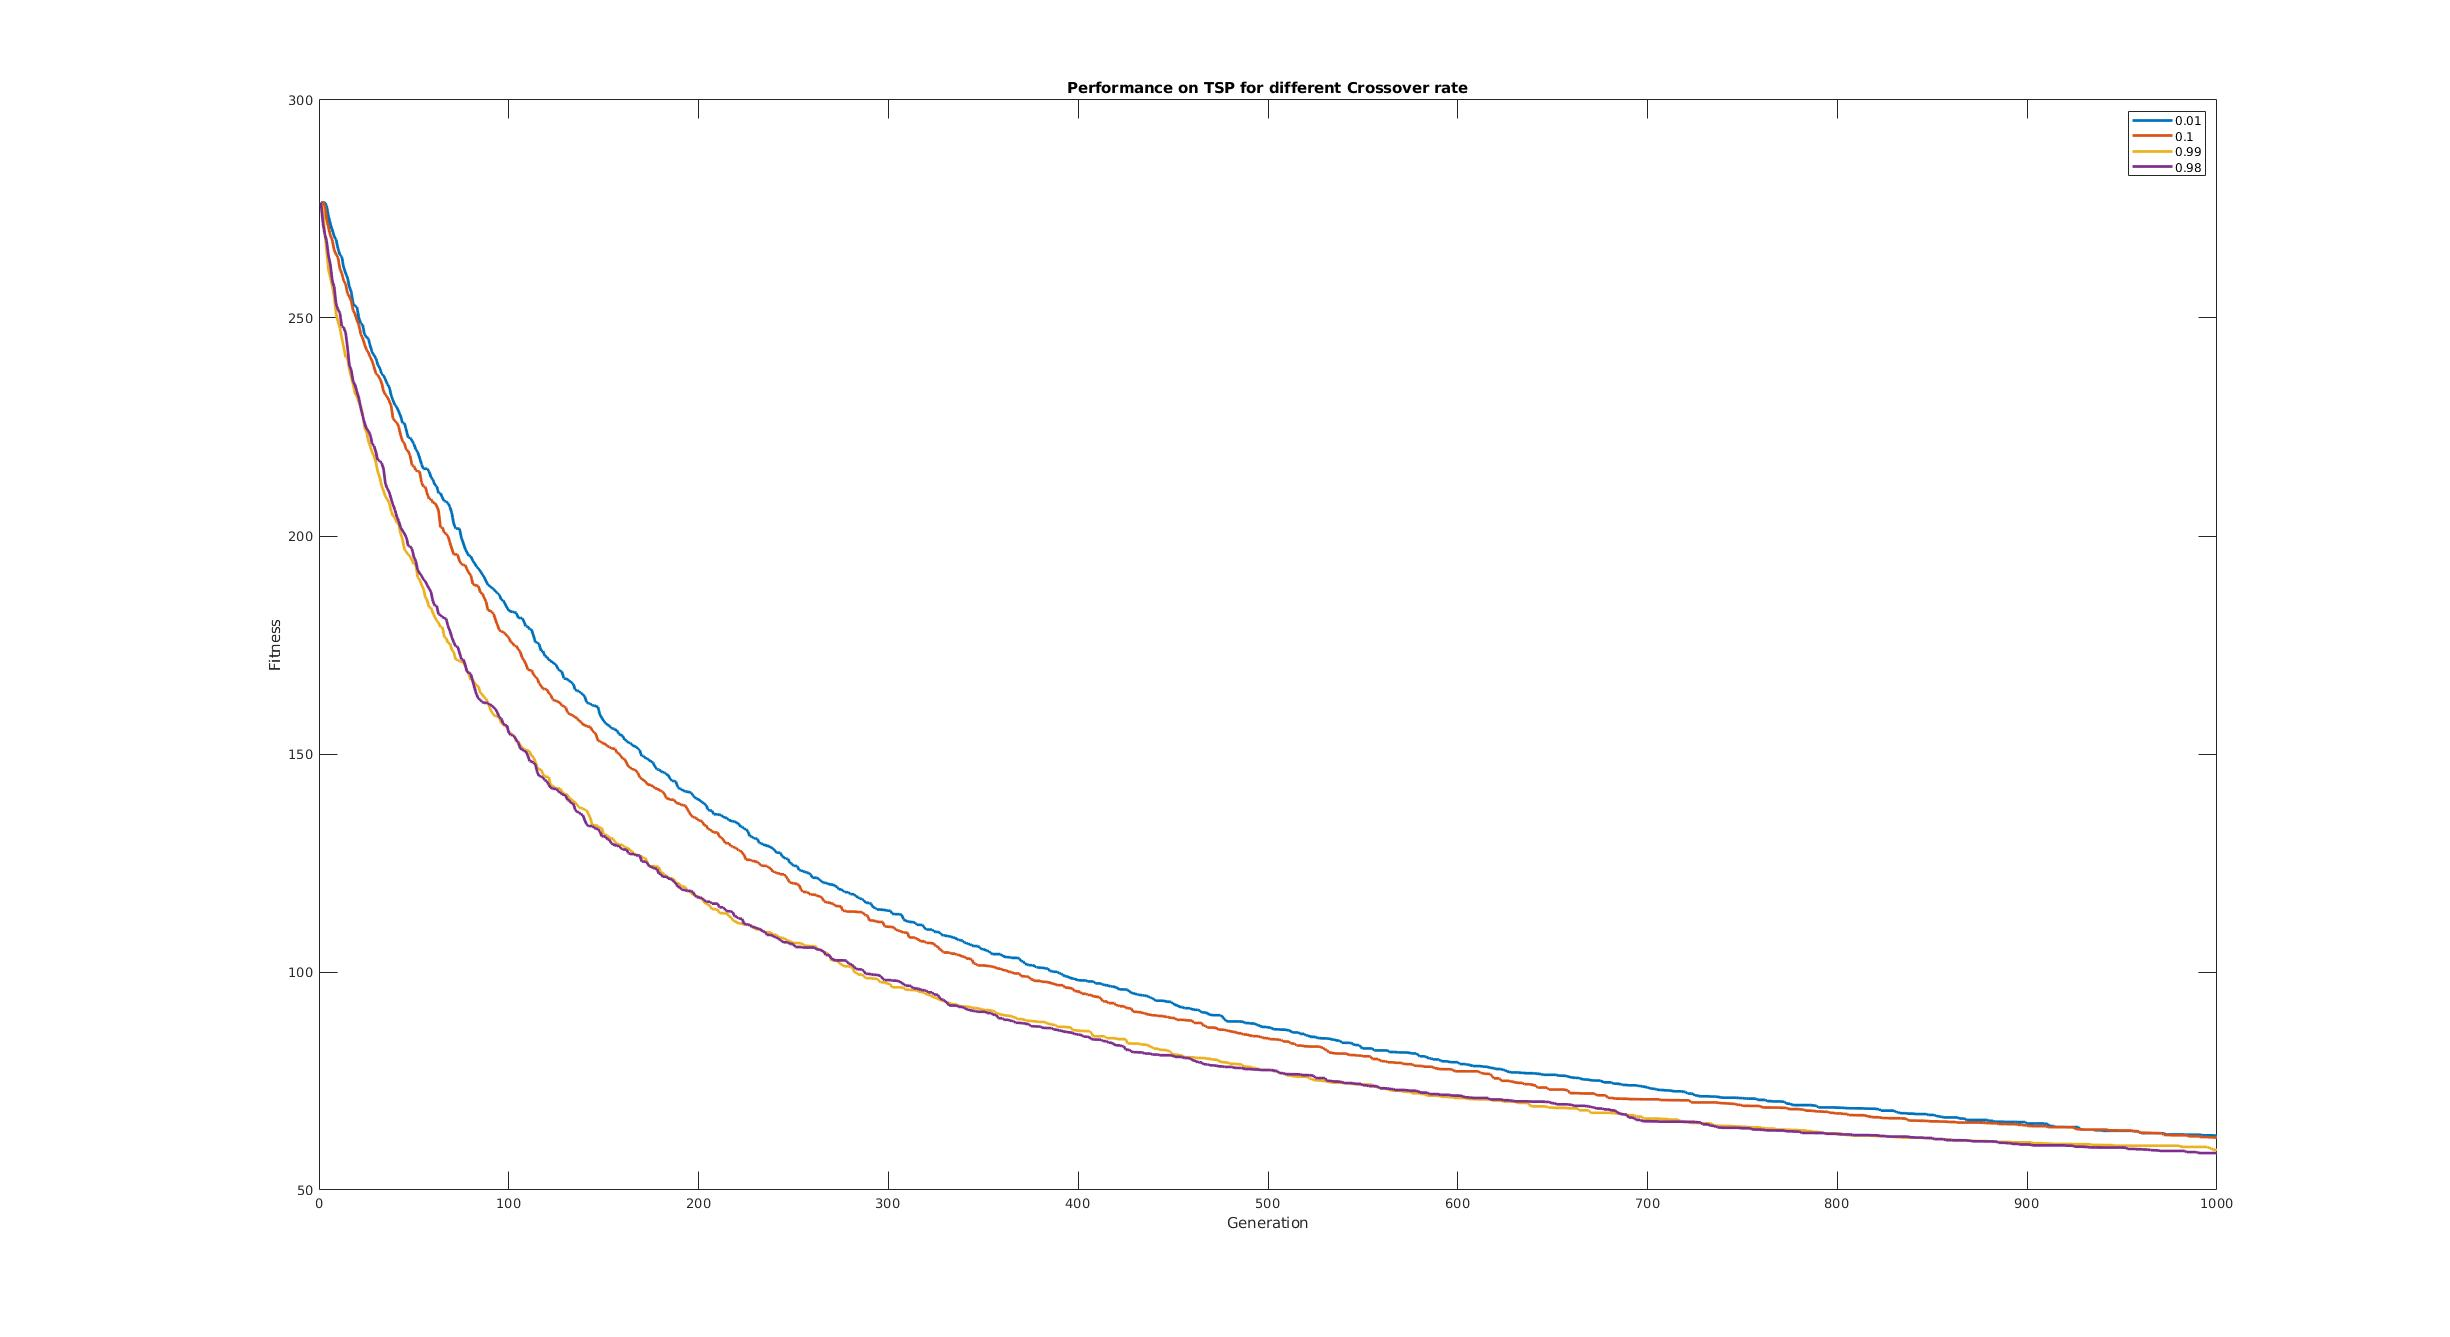
\includegraphics[width=1.0\textwidth]{images/crossover_exp_98.jpg}
	\caption{Crossover rate comparision\label{fig:crossfig}}
\end{figure}

Describe and explain the different mutation rates and how they influence the learning behaviour. Please remember to also focus on why, not only on what.
Also elaborate on the mutation rate you have chosen as best mutation rate.

\newpage

\subsection{Different crossover rates}


\begin{figure}[ht!]
  \centering
  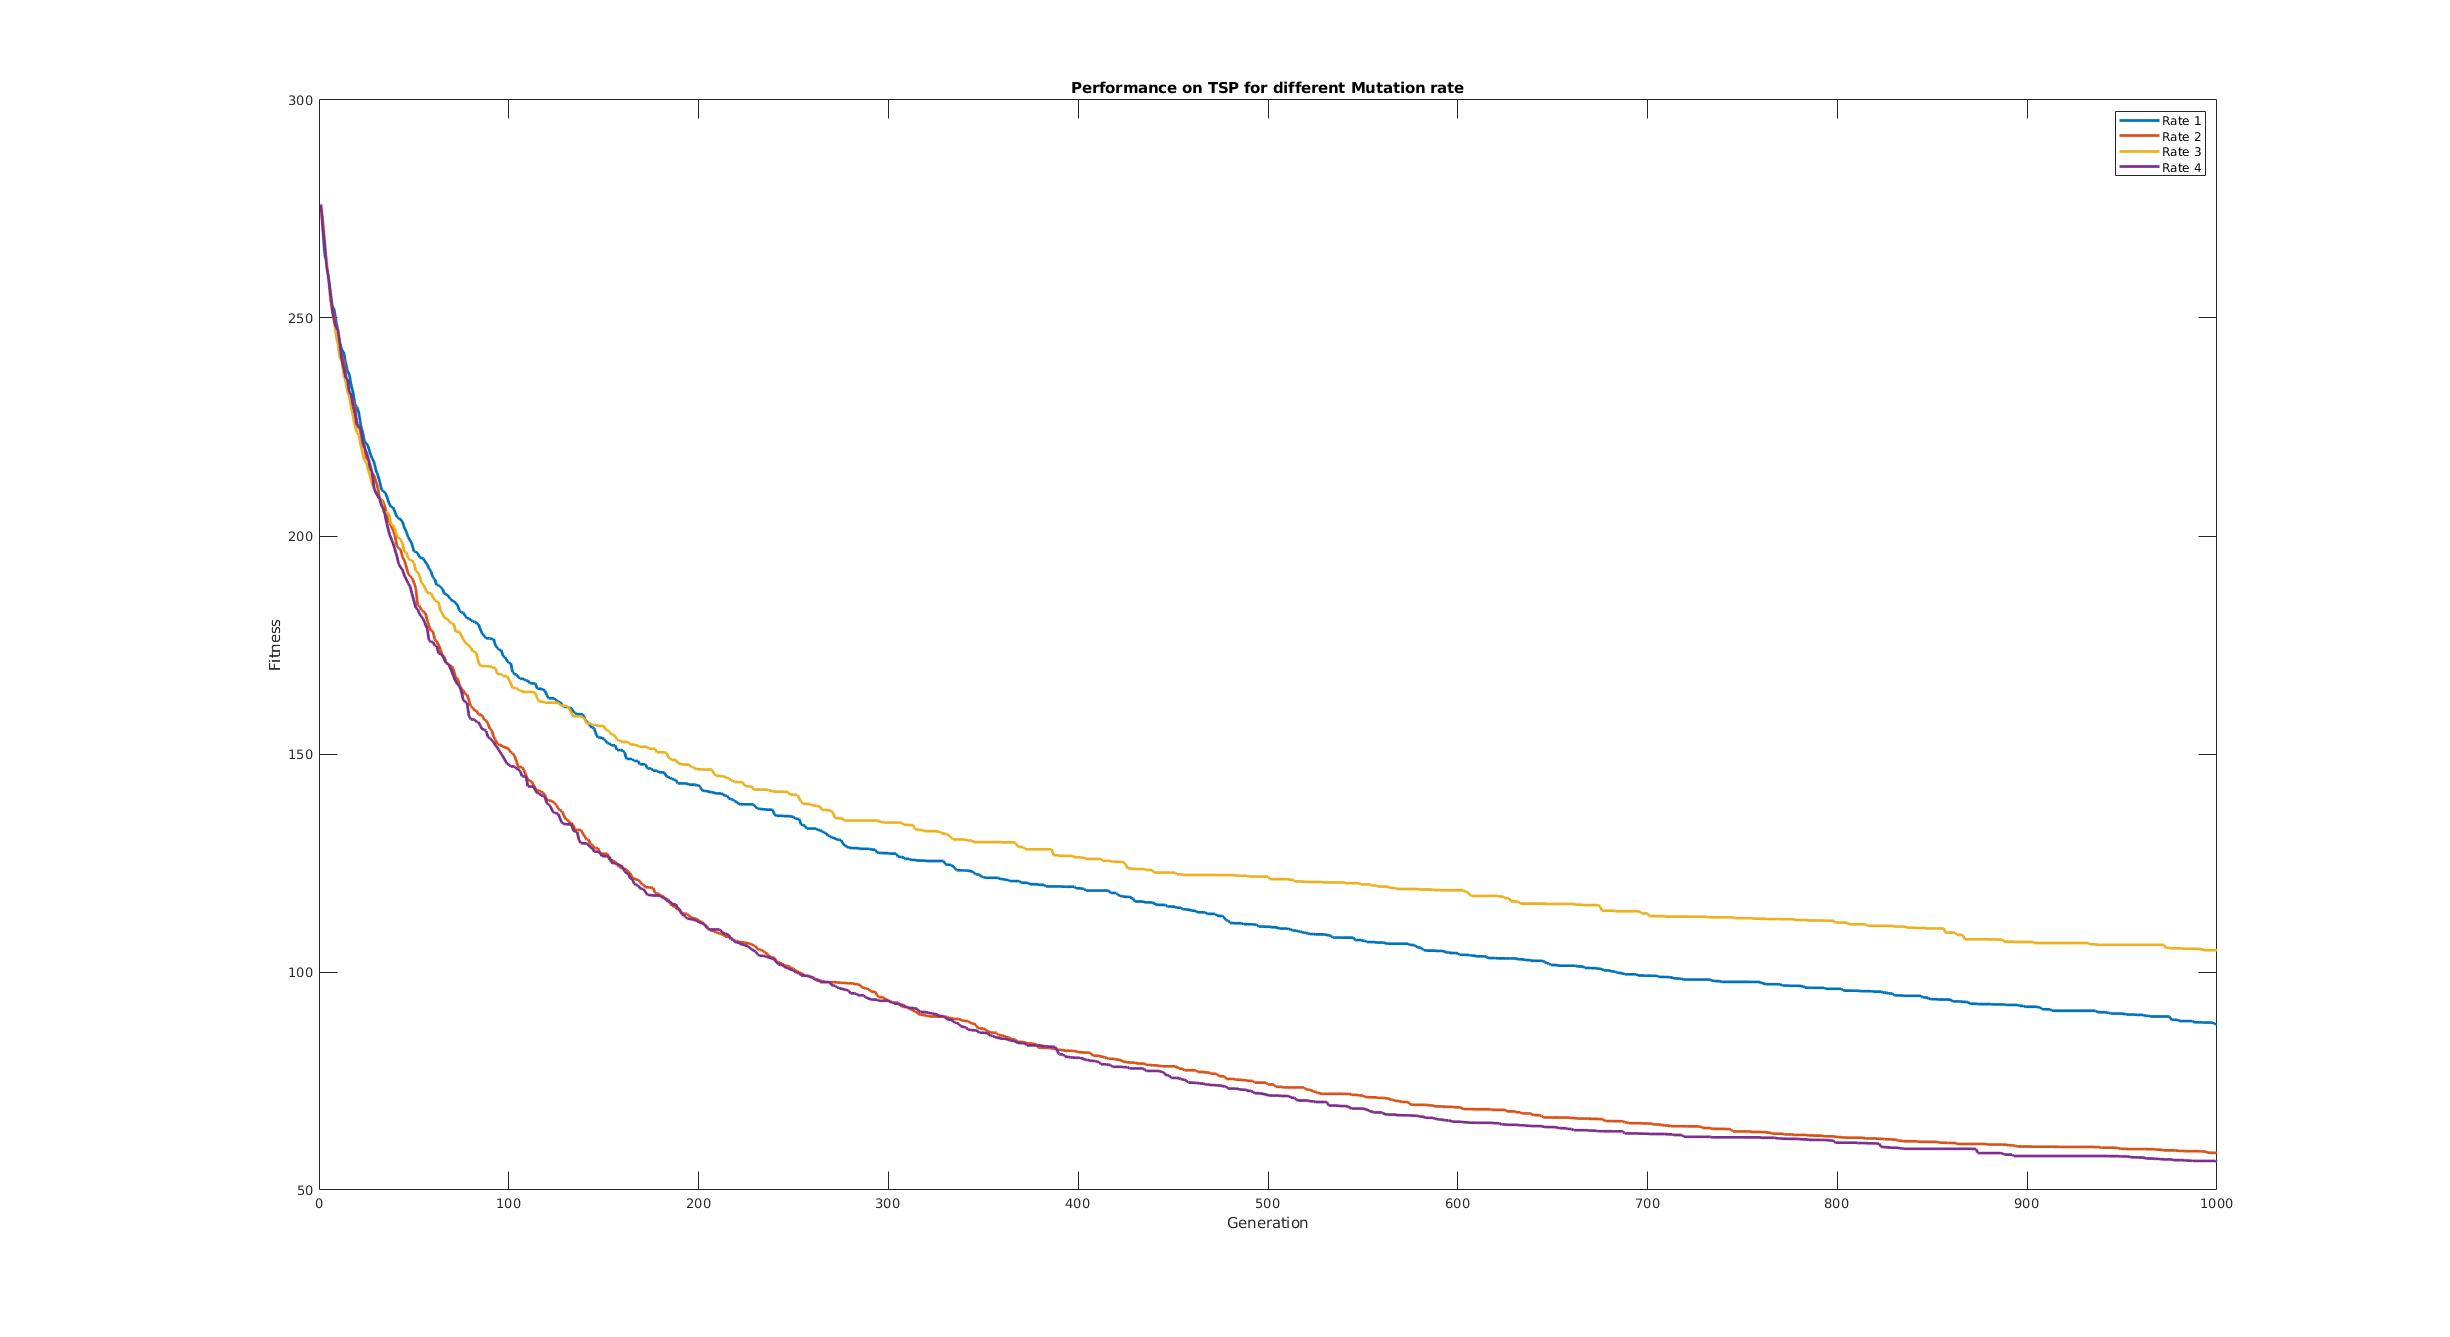
\includegraphics[width=1.0\textwidth]{images/mutation_exp_25.jpg}
    \caption{Mutation rate comparision\label{fig:mutfig}}
\end{figure}

Describe and explain the different crossover rates and how they influence the learning behaviour. Please remember to also focus on why, not only on what.
Also elaborate on the crossover rate you have chosen as best mutation rate.

\begin{figure}[ht!]
  \centering
  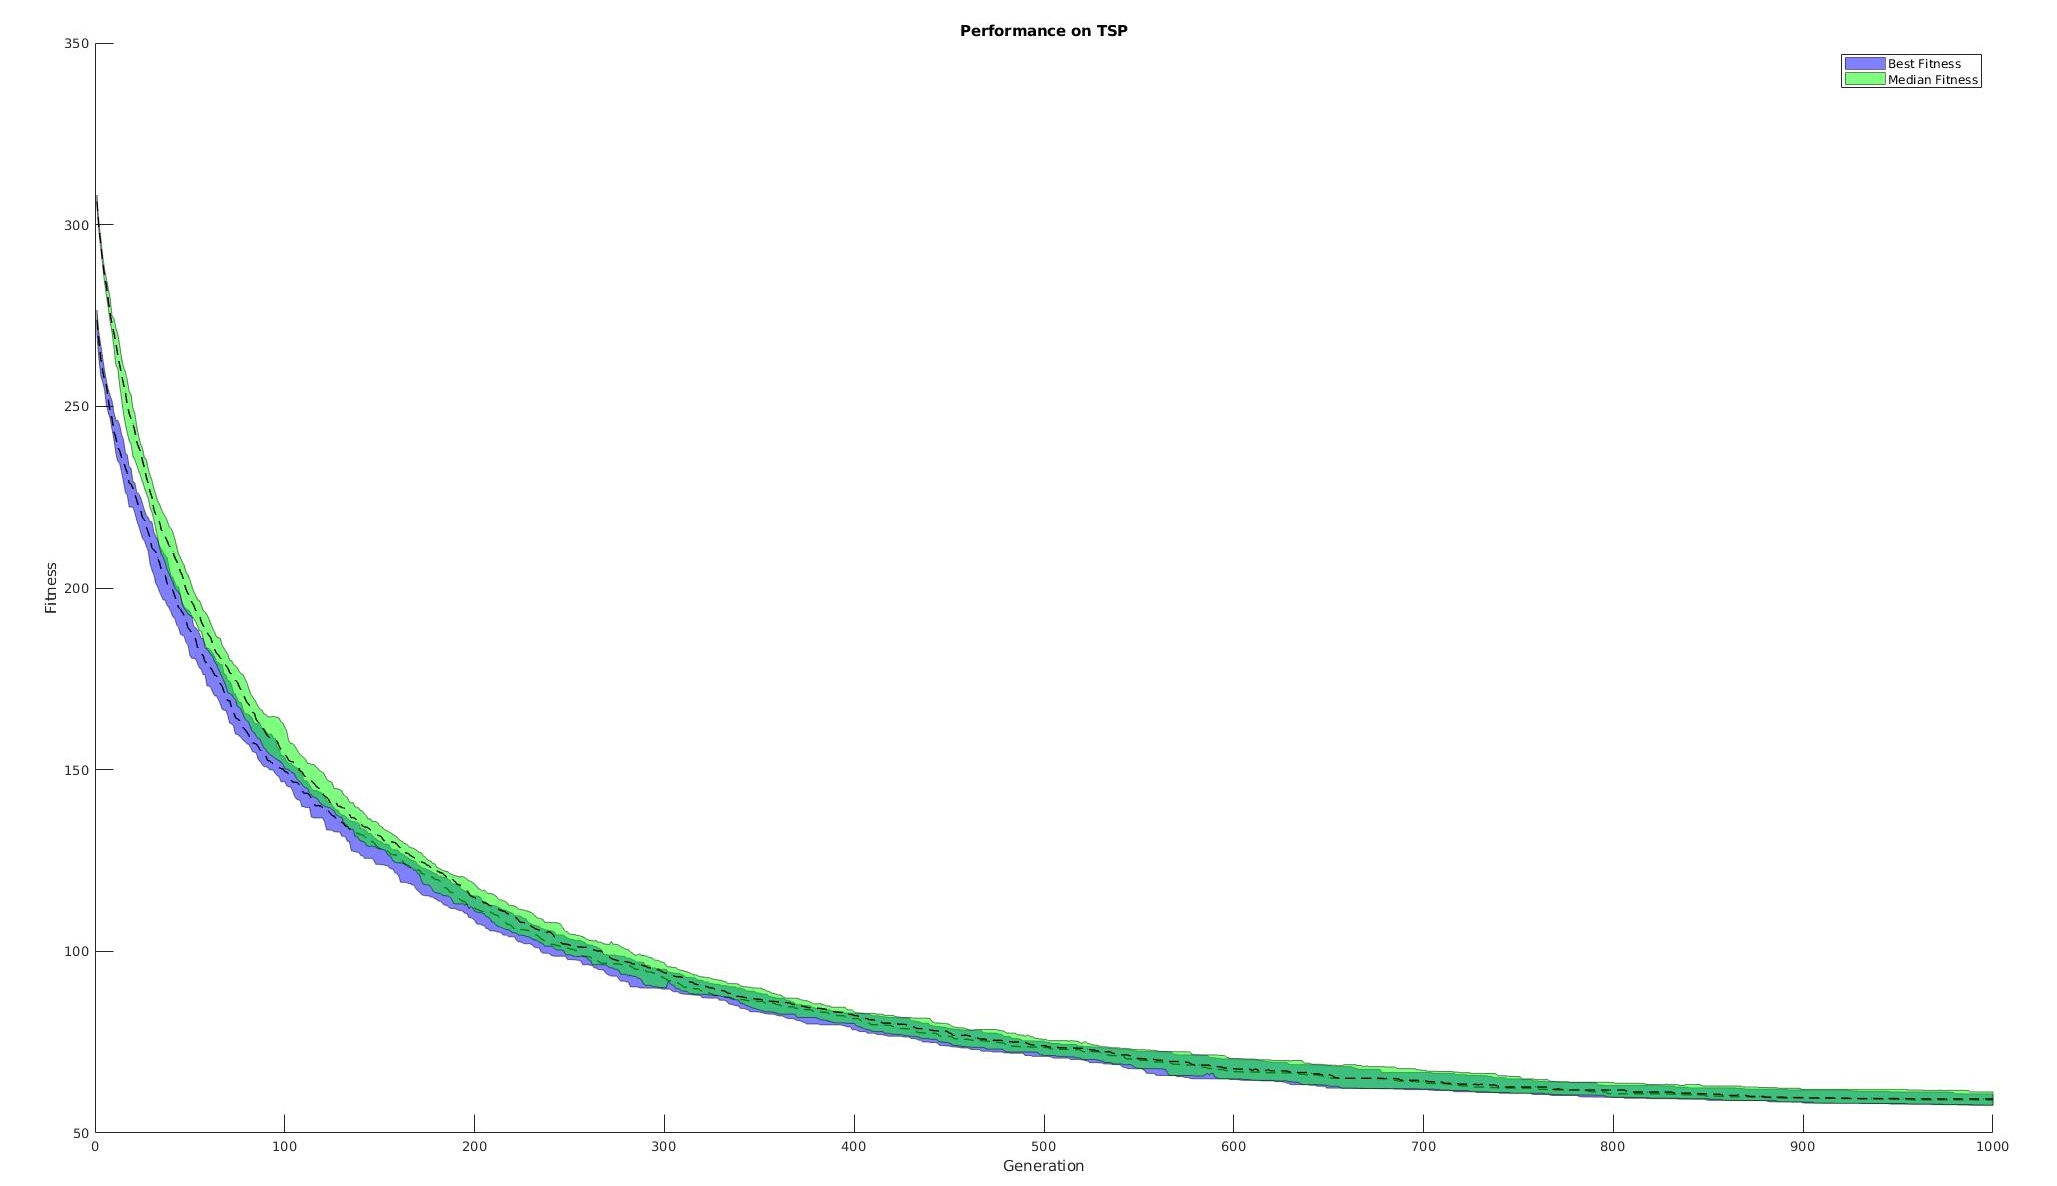
\includegraphics[width=1.0\textwidth]{images/1000X30_updated.jpg}
  \caption{Best and median fitness over 30 Experiments\label{fig:mutfig}}
\end{figure}


\end{document}
